%%%%%%%%%%%%%%%%%%%%%%%%%%%%
% Prototype Implementation %
%%%%%%%%%%%%%%%%%%%%%%%%%%%%

\chapter{Prototyp-Implementierung}
\label{chapter:prototype}

Um den im Kapitel \ref{chapter:interactive-approach} vorgestellten Ansatz für das interaktive Layout von Diagrammen und insbesondere die neu eingeführten Mechanismen für die Interaktion zu validieren, wurde in Rahmen der Arbeit ein Prototyp entwickelt. Mit der Beschreibung des Prototyps beschäftigt sich dieses Kapitel. Im Abschnitt \ref{sec:technologies} wird auf die gewählten Technologien eingegangen. Die Benutzeroberfläche und die unterstützten Funktionen werden im Abschnitt \ref{sec:functions} vorgestellt. Schließlich wird im Abschnitt \ref{sec:architecture} die Architektur des Prototyps thematisiert und einzelne Komponenten beschrieben.

\section{Technologie}
\label{sec:technologies}

Bevor die Entwicklung des Prototyps begonnen hat, wurde nach verfügbaren Komponenten gesucht, die in dem Prototyp verwendet werden könnten. Der umzusetzende Ansatz weist spezielle \textbf{Mechanismen für die Interaktion} auf (siehe Abschnitt \ref{sec:interaction-mechanisms}), die weder in kommerziellen Anwendungen noch in wissenschaftlichen Arbeiten gefunden wurden. Daher lässt sich für die Interaktion keine bestehende Software-Bibliothek einsetzen und die Umsetzung der Mechanismen der Interaktion bildet einen wesentlichen Teil der Entwicklung des Prototyps.

Des Weiteren wurde der Einsatz einer Bibliothek zum \textbf{Graphzeichnen} bedacht. Da die in diesen Bibliotheken bereitgestellte Algorithmen in der Regel eine automatische Berechnung des Layouts durchführen, ist eine Variierung des Layouts durch den Nutzer nicht möglich (siehe Abschnitt \ref{sec:automatic-layout}). Dies ist ebenfalls der Fall beim dem Einsatz dieser Algorithmen in interaktiven Ansätzen. Insbesondere in dem Pattern-basierten Ansatz aus \cite{Maier12A-Pattern-based} ist deutlich zu erkennen, dass sich das Layout nach der Anwendung eines Algorithmus zum Graphzeichnen auf einen gewählten Teil des Diagramms nicht modifizieren lässt (siehe Abschnitt \ref{subsubsec:pattern-based-approach}). Da die Möglichkeit der Layout-Variierung durch den Nutzer eine wichtige Rolle in dem Ansatz spielt, wurde entschieden, die im Abschnitt \ref{subsec:concrete-layout-algorithms} beschriebene Layout-Algorithmen eigenständig zu implementieren. Da es sich um vereinfachte Algorithmen handelt, wurde der Einfachheit halber zu keinem \textbf{Constraintlöser} gegriffen, der z.B. in \textit{Dunnart} eingesetzt wird (siehe Abschnitt \ref{subsubsec:constraint-based-approaches}) und in Form der Software-Bibliothek \textit{Adaptagrams}\footnote{\url{https://github.com/mjwybrow/adaptagrams}} verfügbar ist. Der Einsatz eines Constraintlösers für einen verallgemeinerten Layout-Algorithmus wird im Abschnitt \ref{subsec:algorithm-generalization} diskutiert.

Es wäre denkbar, das \textbf{Layout-Framework aus \cite{Maier12A-Pattern-based}} als Grundlage für die Umsetzung des Prototyps einzusetzen. Dafür wäre es notwendig, die freie Positionierung einzuschränken, z.B. durch das Einführen von impliziten Layout-Patterns. Weiterhin müssten die in \cite{Maier12A-Pattern-based} vorgestellten allgemeinen Layout-Patterns zusammengefasst und um die Möglichkeit der Variierung erweitert werden. Schließlich müsste eine Unterstützung für die Mechanismen der Interaktion geschaffen werden. Da das Layout-Framework zu der Zeit der Anfertigung dieser Bachelor-Arbeit nicht veröffentlicht wurde, war sein Einsatz ausgeschlossen.

Aufgrund der Konzentration auf die Mechanismen der Interaktion und die Bestandteile der Layout-Berechnung wurde das bearbeitete Modell einfach gehalten, das bereits bei der Vorstellung der konkreten Layout-Algorithmen im Abschnitt \ref{subsec:concrete-layout-algorithms} beschrieben wurde. Deshalb war es nicht notwendig, eine verfügbare Implementierung des \textbf{UML-Metamodells} (z.B. Ecore\footnote{\url{http://www.eclipse.org/modeling/emf/}}) zu verwenden.

Da keine Komponenten wiederverwendet werden konnten, wurde eine komplett neue Desktop-Anwendung entwickelt. Es handelt sich um eine native \textbf{Mac OS X Anwendung}, die in der Programmiersprache \textit{Objective-C} entwickelt wurde. Sie verwendet ausschließlich die Standardbibliotheken \textit{Cocoa} und \textit{Quartz} und besitzt keine weiteren Abhängigkeiten.

\section{Funktionen}
\label{sec:functions}

% Anforderungen an den Prototypen?

% kurze Beschreibung des Prototypen
% Screenshot, Demo-Videos auf der DVD
% Implementierte Funktionalität
% unterstützte Aktionen und Layout-Methoden (Auswahl möglich)
% welcher Teil wurde umgesetzt?

% einfach gehalten

\section{Architektur}
\label{sec:architecture}

% Präfix "IDL" erklären
% Umfang der Implementierung
% keine Frameworks, nur logische Aufteilung des Codes

\subsection{Layout Engine}

% Diagramm!

\subsubsection{Geometry}

% Koordinaten-Konversion mit Bild (NSView vs. IDLLayoutEngine)
% zentrierte Koordinaten -> Förderung der Umsetzung des impliziten Patterns zur Zentrierung

\subsubsection{Diagram}
\label{subsubsec:component-diagram}

% aus zeitlichen Gründen wurde die Semantik nicht tiefgründig ausgearbeitet und wurde der weiteren Forschung überlassen
% kein Metamodell
% keine Unterscheidung der abstrakten und konkreten Syntax

% IDLEdge -> gerichtete Kanten mit max. einem Elternknoten (z.B. Vererbung in Klassendiagrammen) -> Diagramm ist also azyklisch

\subsubsection{Layout}

\subsubsection{Patterns}

% nur expliziten
% wie werden die impliziten Patterns im Prototypen implementiert -> durch die konkreten IDLLayoutEngine's
% Wiederverwendung, Komposition in IDLTShapePattern

\begin{figure}[hbt]
    \centering
    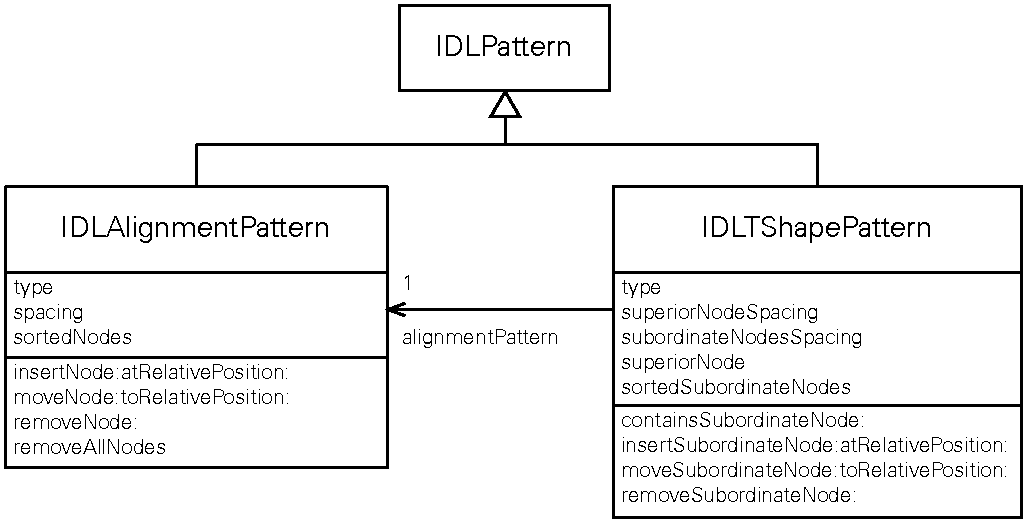
\includegraphics[width=\textwidth]{resources/layout-patterns-implementation}
    \caption{}
    \label{fig:layout-patterns-implementation}
\end{figure}

\subsubsection{Events}

\subsubsection{Engine}

% IDLLayoutEngine & Subclasses (bzw. unterstützte Layout-Engines)

% IDLLayoutEngine besitzt intern Referenzen auf den Inhalt des Diagramms und muss daher mit dem Diagramm synchronisiert werden (manuell) mit s.g. Layout-Events

% Löschen eines (oder mehreren Elementen) im Prototypen nicht unterstützt, nur hinzufügen und "rausfahren"

\subsection{Canvas View}

% Animation der Layout-Übergängen
% - implizite Core Animation Animation
% - Überführen von mehreren Animationen mit POP => wichtiger in Multi-Touch-Umgebung, bei Desktop nur ein Mauszeiger, keine parallele Aktionen

% Vergrößerung des Fensters -> Zentrierung des Inhalts (durch die Umrechnung)

% Berechnung der Start- und Endpunkte der Kanten anhand von Eigenschaften der Knoten (siehe OmniGraffle)

\subsection{Dragging Manager}

% Drag and Drop

\subsection{Application}
